\section{Introduction}

\begin{frame}{Tobacco Cessation and AI Support}
    \begin{columns}[c]
        \column{.55\textwidth}
        \textbf{The Challenge of Tobacco Cessation}
        \begin{itemize}
            \item 1.3 billion tobacco users worldwide
            \item Only 30\% of cessation attempts succeed
            \item Limited access to personalized support
            \item Types of support:
            \begin{itemize}
                    \item \textbf{Behavioral counseling}: Limited availability
                    \item \textbf{Medication}: Not accessible to all
                    \item \textbf{Digital interventions}:     Often generic
        \end{itemize}
            \item \textbf{Our solution}: AI-powered personalized cessation support through SmokeCtrl
        \end{itemize}
        
        \column{.45\textwidth}
        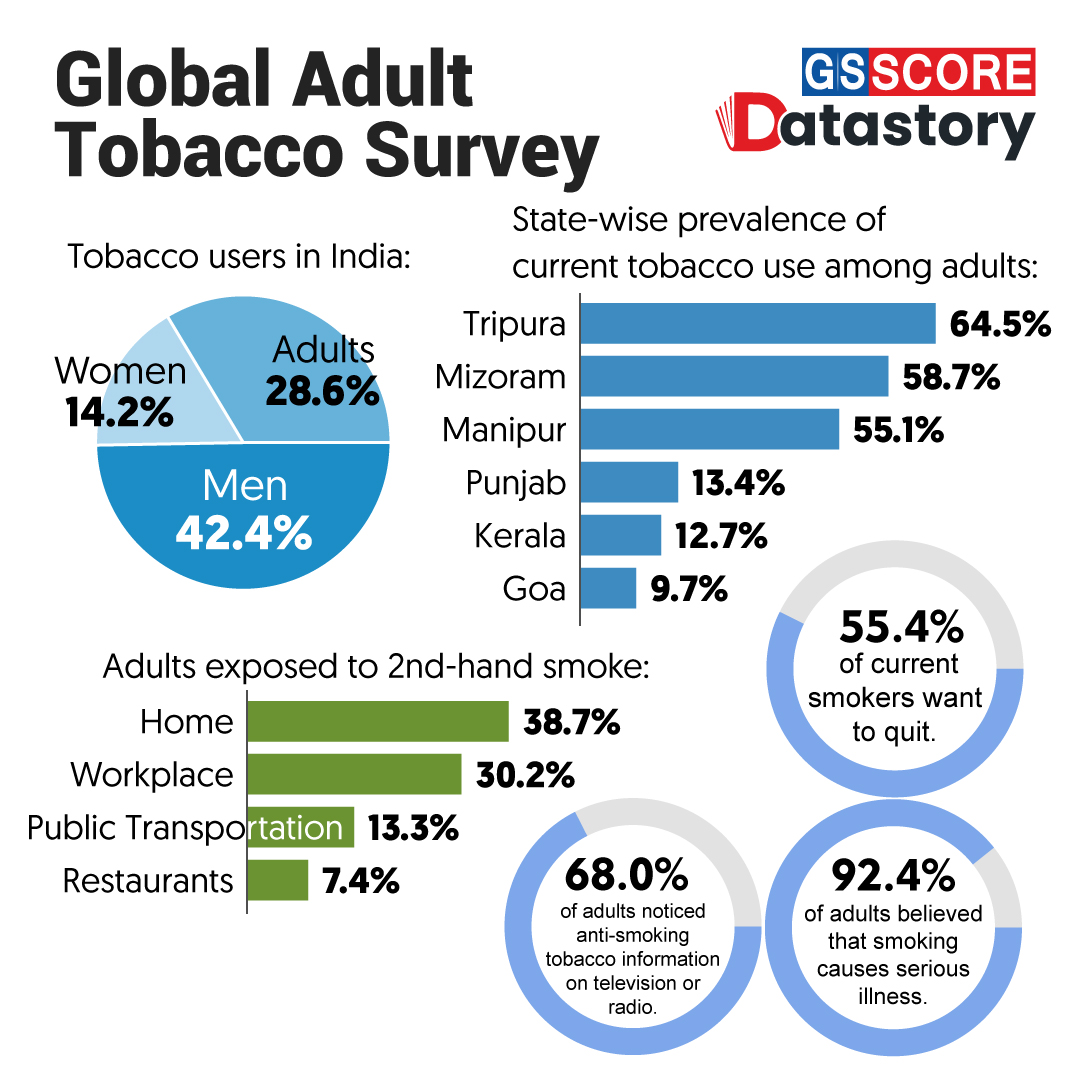
\includegraphics[width=0.75\linewidth, height=5cm]{presentation/images/Introduction/tobacco_stats.jpg}
    \end{columns}
\end{frame}

\begin{frame}{Our Chief Contributions}
  \begin{itemize}
    \item \textbf{Multimodal intervention platform}: Mobile-accessible LLMs for tobacco cessation
    
    \item \textbf{Agent-based synthetic dialogue framework}: Domain-specific conversations with explicit reasoning
    
    \item \textbf{Retrieval-augmented inference}: Enhanced contextual relevance via vector-based knowledge
    
    \item \textbf{Parameter-efficient adaptation}: Quantized low-rank fine-tuning for domain specialization
    
    \item \textbf{Empirical validation}: Demonstrated synthetic data efficacy for clinical accuracy
    
    \item \textbf{Novel discourse initiation}: Solutions for cold-start challenges in therapeutic agents
  \end{itemize}
\end{frame}